W przypadku standardowego modelu z walidacją krzyżową model bardzo szybko uległ przeuczeniu.
Już po szóstej iteracji dokładność na zbiorze walidaycjnym wyniosła 100\%, co nie jest realistycznie możliwe.
Została podjęta próba ograniczenia przeuczenia poprzez zwiększenie zbioru danych, zmiany liczby epok w modelu
oraz manipulacji współczynnikami dropout i regularyzacji.
W każdym przypadku model zwracał niezadowalające wyniki wynoszące 100\% po jednej z początkowych iteracji.

\begin{figure}[ht]
	\centering
	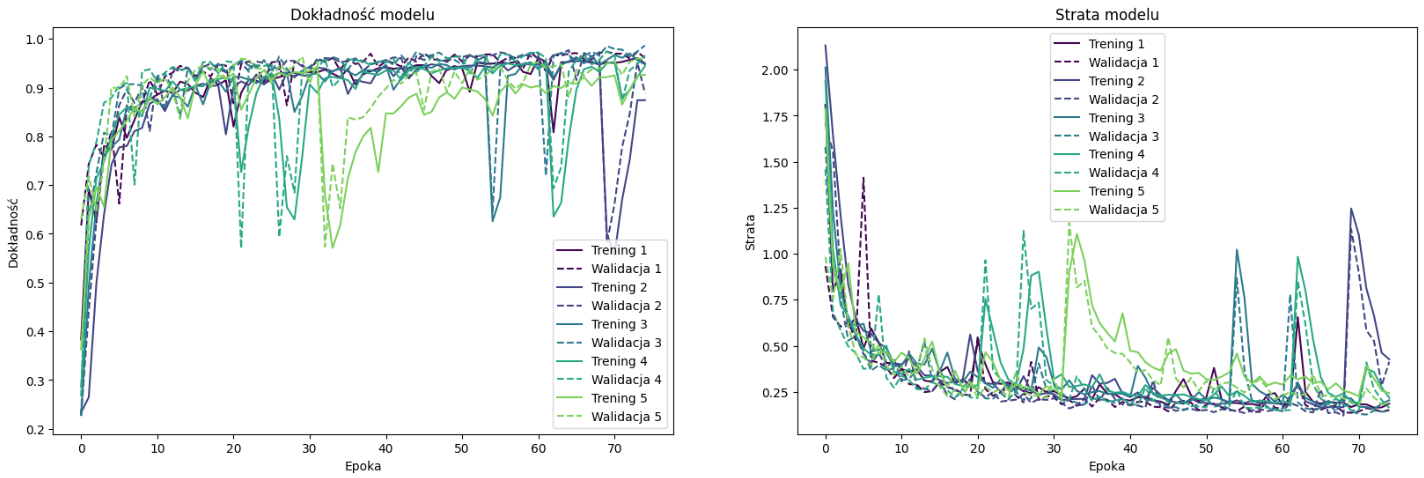
\includegraphics[height=5.5cm]{resources/tests/images/v3/crossvalid_img.png}
	\caption{Wyniki testów dla modelu z walidacją krzyżową}
	\label{Fig:tests-cv-1}
\end{figure}
\FloatBarrier

Z powodu przeuczenia model nie radził sobie z zewnętrznymi obrazkami testowymi.
Większość grafów określił jako grafy pełne, co nie jest zgodne ze stanem rzeczywistym.

\begin{figure}[ht]
	\centering
	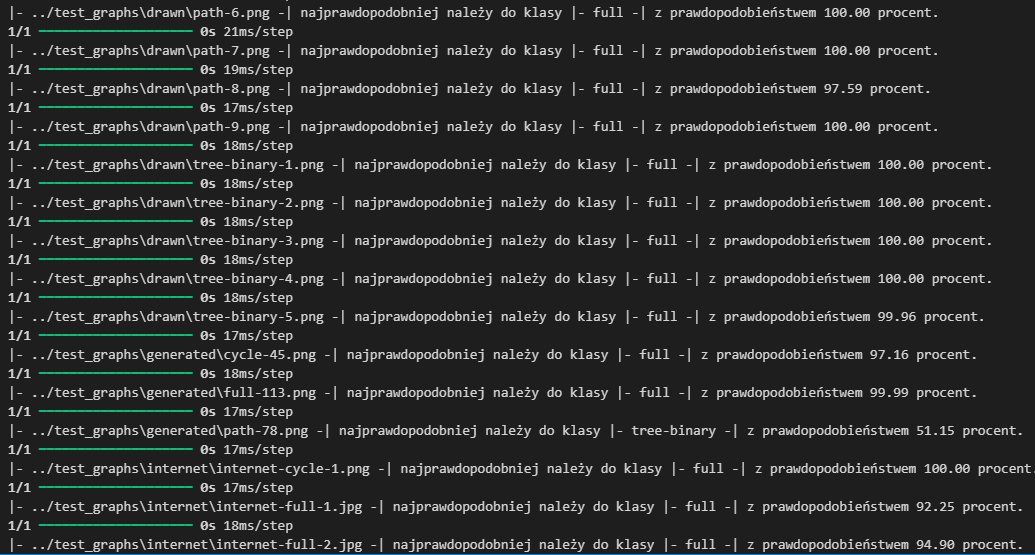
\includegraphics[height=7cm]{resources/tests/images/v3/crossvalid_txt.png}
	\caption{Klasyfikacja obrazów zewnętrznych dla modelu z walidacją krzyżową}
	\label{Fig:tests-cv-2}
\end{figure}
\FloatBarrier